\chapter{Результаты}
\label{ch:results}

\section{Текстовая документация}
Один из наиболее распространенных форматов представления результатов проекта - это документация в виде текстового документа. Однако текстовый формат может быть не очень наглядным и неудобным для понимания, особенно для людей, не имеющих технического образования.

Для представления результатов проекта в виде документации можно использовать различные форматы текстовых документов, такие как отчеты, статьи, обзоры и т.д. Важно, чтобы документация была структурированной, легко читаемой и визуально привлекательной для аудитории.

В текстовом документе результаты проекта обычно представляются в следующей структуре:
\begin{enumerate}
    \item Введение
        \begin{itemize}
            \item Обзор проекта и его целей
            \item Краткое описание методологии работы
        \end{itemize}
    \item Методология
        \begin{itemize}
            \item Описание используемых методов и техник
            \item Обоснование выбора методологии
        \end{itemize}
    \item Результаты и анализ
        \begin{itemize}
            \item Подробное описание полученных результатов
            \item Визуализация данных (графики, таблицы и диаграммы)
            \item Анализ результатов и выводы
        \end{itemize}
    \item Примеры реализации
        \begin{itemize}
            \item Показ примеров успешной реализации проекта
            \item Описание преимуществ и достижений
        \end{itemize}
    \item Выводы и рекомендации
        \begin{itemize}
            \item Общая оценка результатов проекта
            \item Рекомендации для дальнейшей работы или улучшения проекта
        \end{itemize}
    \item Заключение
        \begin{itemize}
            \item Подведение итогов и обобщение результатов
            \item Благодарности участникам и заинтересованным сторонам
        \end{itemize}
\end{enumerate}

\subsection*{Преимущества}
Представление результатов проекта в виде документации в текстовом формате имеет ряд преимуществ

\begin{enumerate}
\item Наглядность и визуализация:
    \begin{itemize}
        \item Презентация позволяет эффективно визуализировать ключевые моменты, используя слайды с графиками, диаграммами, схемами и другими иллюстративными элементами.
        \item Это помогает лучше донести информацию и повысить понимание аудитории.
    \end{itemize}
\item Структурированность и логичность:
    \begin{itemize}
        \item Презентация предполагает наличие четкой структуры, включающей введение, основную часть и заключение.
        \item Это способствует последовательному изложению и логичному представлению хода решения задачи.
    \end{itemize}
\item Акцент на главное:
    \begin{itemize}
        \item Презентация позволяет выделить и сфокусировать внимание аудитории на ключевых моментах, результатах и выводах.
        \item Это помогает эффективно передать основную идею и избежать перегрузки деталями.
    \end{itemize}
\item Интерактивность и вовлечение аудитории:
    \begin{itemize}
        \item Презентация предоставляет возможность для интерактивного взаимодействия с аудиторией, например, через вопросы и ответы, обсуждение слайдов.
        \item Это способствует активному участию и вовлечению аудитории в процесс.
    \end{itemize}
\item Гибкость и адаптируемость:
    \begin{itemize}
        \item Презентацию можно легко адаптировать под конкретную аудиторию, ее уровень подготовки и интересы.
        \item Можно сделать акцент на различных аспектах решения в зависимости от потребностей.
    \end{itemize}
\end{enumerate}

\subsection*{Недостатки}
\begin{enumerate}
    \item Ограниченность по объему:
        \begin{itemize}
            \item Презентация обычно не позволяет подробно освещать все аспекты решения задачи, так как ограничена во времени и количестве слайдов.
            \item Это может привести к упущению важных деталей или недостаточной глубине проработки.
        \end{itemize}
    \item Возможность перегрузки информацией:
        \begin{itemize}
            \item Существует риск, что презентация будет перегружена текстом, графиками и деталями, что может отвлекать и утомлять аудиторию.
            \item Необходим баланс между визуальной информативностью и лаконичностью.
        \end{itemize}
    \item Зависимость от технических средств:
        \begin{itemize}
            \item Презентация требует наличия соответствующего оборудования (проектор, компьютер) и работоспособности программного обеспечения.
            \item Возможны технические сбои, что может нарушить ход представления результатов.
        \end{itemize}
    \item Отсутствие детальной документации:
        \begin{itemize}
            \item Презентация сама по себе не является полноценной документацией и не может заменить более подробные технические отчеты или руководства.
            \item Для полноты картины может потребоваться предоставление дополнительной документации.
        \end{itemize}
    \item Сложность внесения изменений:
        \begin{itemize}
            \item Внесение изменений в презентацию после ее создания может быть более трудоемким по сравнению с другими форматами представления результатов.
        \end{itemize}
\end{enumerate}

Таким образом, презентация является эффективным форматом для наглядного и структурированного представления ключевых моментов решения задачи, но она должна быть дополнена другими форматами для обеспечения всесторонней документации и обмена информацией.

\section{Интерактивное представление}
Интерактивные элементы для представления результатов проекта могут быть очень эффективным способом вовлечения и взаимодействия с аудиторией. Рассмотрим подробнее этот формат
\begin{enumerate}
    \item Создание интерактивных прототипов, макетов или демонстрационных версий
        \begin{itemize}
            \item Интерактивные прототипы позволяют создавать интерактивные модели будущего приложения или системы.
            \item Они могут включать в себя элементы пользовательского интерфейса, навигацию, логику работы и другие функциональные компоненты.
            \item Такие прототипы помогают наглядно продемонстрировать основные возможности и принципы работы разработанного решения.
        \end{itemize}
    \item Взаимодействие аудитории с интерактивными элементами
        \begin{itemize}
            \item Интерактивные прототипы или демонстрационные версии позволяют аудитории напрямую взаимодействовать с результатами проекта.
            \item Слушатели могут самостоятельно попробовать использовать ключевые функции, проверить логику работы, оценить удобство использования.
            \item Такое интерактивное взаимодействие помогает лучше понять и прочувствовать полученные результаты.
            \item Аудитория может оставлять обратную связь, предлагать идеи и видеть, как реагирует прототип на их действия.
        \end{itemize}
    \item Реализация интерактивных элементов
        \begin{itemize}
            \item Интерактивные прототипы и демонстрационные версии могут быть реализованы с использованием различных технологий и инструментов:
            \item Веб-технологии, такие как HTML, CSS, JavaScript, обеспечивают высокую степень интерактивности и кроссплатформенность.
            \item Мобильные приложения позволяют создавать интерактивные демонстрации, максимально приближенные к реальному продукту.
            \item Специализированные инструменты для создания интерактивных прототипов, например, Figma, Adobe XD, InVision, предоставляют удобные средства для быстрого создания и демонстрации интерактивных моделей.
            \item Выбор технологий и инструментов зависит от специфики проекта, требований к демонстрации и доступных ресурсов.
        \end{itemize}
\end{enumerate}

\subsection*{Преимущества}
Использование интерактивных элементов при представлении результатов проекта по программированию имеет ряд преимуществ
\begin{enumerate}
    \item Повышение вовлеченности и интереса аудитории:
        \begin{itemize}
            \item Интерактивные демонстрации и прототипы позволяют аудитории непосредственно взаимодействовать с разработанным решением.
            \item Возможность самостоятельно испытать и опробовать функциональность вызывает больший интерес и вовлеченность слушателей.
            \item Это помогает избежать пассивного восприятия и повышает их заинтересованность в проекте.
            \item Вовлеченная аудитория лучше воспринимает и запоминает представленную информацию.
        \end{itemize}
    \item Обеспечение более глубокого понимания функциональности и принципов работы:
        \begin{itemize}
            \item Интерактивные элементы дают возможность аудитории самостоятельно исследовать и изучить работу системы.
            \item Слушатели могут попробовать различные функции, проверить логику, взаимодействие между компонентами.
            \item Такое активное взаимодействие способствует лучшему пониманию внутренних механизмов и принципов реализации решения.
            \item Аудитория может оценить удобство использования, выявить особенности и нюансы работы системы.
        \end{itemize}
    \item Получение непосредственной обратной связи:
        \begin{itemize}
            \item Интерактивные демонстрации позволяют получать прямую реакцию и отзывы от аудитории.
            \item Слушатели могут высказывать свои комментарии, предложения и пожелания по улучшению представленного решения.
            \item Такая обратная связь дает ценную информацию, которую можно использовать для дальнейшего совершенствования продукта.
            \item Интерактивное взаимодействие помогает выявить ключевые проблемы, недостатки или области для улучшения.
        \end{itemize}
        \item Демонстрация технических возможностей и навыков команды:
        \begin{itemize}
            \item Использование интерактивных элементов при представлении результатов проекта демонстрирует технические возможности и навыки команды разработчиков.
            \item Это показывает, что команда способна создавать не только функциональное, но и интерактивное, отзывчивое и высококачественное программное обеспечение.
            \item Интерактивные демонстрации позволяют выделить и подчеркнуть ключевые технические достижения и компетенции команды.
            \item Это может вызвать больший интерес и доверие у аудитории,а также привлечь внимание потенциальных заказчиков или партнеров.
        \end{itemize}
\end{enumerate}

Использование интерактивных элементов предоставляет значительные преимущества в контексте представления результатов проекта. Это помогает вовлечь аудиторию, обеспечить более глубокое понимание решения, получить ценную обратную связь и продемонстрировать технические возможности команды.

\subsection*{Недостатки}
Несмотря на множество преимуществ, использование интерактивных элементов при представлении результатов проекта по программированию также имеет некоторые недостатки, которые стоит учитывать:
\begin{enumerate}
    \item Дополнительные затраты ресурсов:
        \begin{itemize}
            \item Разработка качественных интерактивных демонстраций или прототипов требует дополнительных временных и финансовых затрат.
            \item Команде необходимо выделить ресурсы на проектирование, разработку и тестирование интерактивных компонентов.
            \item Это может повлиять на общий бюджет и сроки реализации основного проекта.
        \end{itemize}
    \item Необходимость в специальных навыках:
        \begin{itemize}
            \item Создание интерактивных элементов предполагает наличие специальных навыков у членов команды, таких как веб-разработка, прототипирование, UI/UX-дизайн.
            \item Если в команде нет специалистов с соответствующей квалификацией, потребуется привлечение дополнительных ресурсов или обучение существующих сотрудников.
            \item Это накладывает дополнительную нагрузку на команду и может замедлить процесс подготовки к представлению результатов.
        \end{itemize}
    \item Риск технических проблем:
        \begin{itemize}
            \item Интерактивные демонстрации и прототипы могут быть более чувствительны к техническим проблемам, таким как несовместимость с различными устройствами или средами, ошибки в работе, проблемы производительности.
            \item Эти технические сложности требуют тщательного тестирования и отладки, чтобы обеспечить стабильную работу интерактивных элементов.
            \item Возникновение технических проблем во время презентации может негативно повлиять на впечатление аудитории.
        \end{itemize}
    \item Отвлечение внимания от основных результатов:
        \begin{itemize}
            \item Чрезмерный фокус на интерактивных элементах может отвлекать аудиторию от ключевых результатов и выводов проекта.
            \item Слушатели могут быть настолько заинтересованы в тестировании интерактивной демонстрации, что упустят важную информацию об основных достижениях.
            \item Необходимо найти баланс между интерактивными элементами и эффективным представлением итогов проекта.
        \end{itemize}
    \item Уместность использования:
        \begin{itemize}
            \item Команда должна оценить, насколько целесообразно инвестировать время и усилия в интерактивные элементы по сравнению с другими формами представления.
        \end{itemize}
\end{enumerate}

Таким образом, создание качественных интерактивных элементов может потребовать дополнительных усилий и ресурсов. Важно найти баланс между интерактивностью и простотой демонстрации, чтобы обеспечить максимальную эффективность представления результатов.

\section{Интерпретация результатов}
Интерпретация результатов проекта является важным завершающим этапом, позволяющим извлечь максимальную ценность из проделанной работы.
\begin{enumerate}
    \item Анализ достижения целей:
        \begin{itemize}
            \item Оценить, насколько успешно были достигнуты поставленные цели и задачи проекта.
            \item Выявить, какие ключевые результаты были получены в ходе реализации проекта.
            \item Определить, в какой степени реализованное решение соответствует первоначальным требованиям и ожиданиям.
        \end{itemize}
    \item Выявление ключевых выводов:
        \begin{itemize}
            \item Сформулировать основные выводы, которые можно сделать на основе полученных результатов.
            \item Проанализировать, какие закономерности, тенденции или инсайты удалось выявить в ходе проекта.
            \item Определить, какие новые знания или понимание были получены в результате проведенной работы.
        \end{itemize}
    \item Оценка ценности и значимости:
        \begin{itemize}
            \item Рассмотреть, какую практическую ценность и преимущества несет разработанное решение.
            \item Оценить, как внедрение результатов проекта может повлиять на бизнес-показатели, эффективность процессов или удовлетворенность пользователей.
            \item Определить, насколько значимым и актуальным является разработанное решение для целевой аудитории.
        \end{itemize}
    \item Выявление областей улучшения:
        \begin{itemize}
            \item Проанализировать, какие аспекты решения требуют доработки или дополнительной проработки.
            \item Определить ключевые ограничения, недостатки или проблемы, выявленные в ходе реализации проекта.
            \item Сформулировать рекомендации по дальнейшему развитию и совершенствованию проекта.
        \end{itemize}
    \item Обобщение и систематизация:
        \begin{itemize}
            \item Свести полученные результаты в единую систему, выделяя взаимосвязи и ключевые взаимозависимости.
            \item Рассмотреть результаты в более широком контексте, соотнося их с отраслевыми тенденциями или стратегическими целями организации.
            \item Сформулировать обобщенные заключения и выводы, которые могут быть применимы и в других проектах.
        \end{itemize}
\end{enumerate}

Эффективная интерпретация результатов позволяет не только представить итоги проектной работы, но и извлечь максимальную ценность из полученных данных. Это помогает лучше понять достигнутые результаты, их значение и перспективы дальнейшего развития.

\section{Оценка}
Существует несколько основных подходов к оценке результатов проекта:
\begin{enumerate}
    \item Сравнение с целевыми показателями:
        \begin{itemize}
            \item Определение степени достижения поставленных целей и задач проекта.
            \item Сопоставление фактических результатов с запланированными целевыми значениями.
            \item Расчет процента выполнения каждой из целей.
        \end{itemize}
    \item Анализ ключевых метрик и индикаторов:
        \begin{itemize}
            \item Выявление и измерение ключевых показателей, характеризующих успешность проекта.
            \item Примеры метрик: время на разработку, затраты, количество новых пользователей, производительность и т.д.
            \item Сравнение фактических значений с плановыми, оценка динамики изменения.
        \end{itemize}
    \item Оценка соответствия требованиям:
        \begin{itemize}
            \item Проверка того, насколько реализованное решение отвечает изначальным техническим требованиям и спецификациям.
            \item Сопоставление характеристик и функциональности продукта с ожидаемыми.
            \item Выявление возможных несоответствий или отклонений.
        \end{itemize}
    \item Экспертная оценка качества:
        \begin{itemize}
            \item Привлечение экспертов и специалистов для оценки достигнутых результатов.
            \item Экспертная оценка может быть основана на демонстрации, тестировании, рецензировании.
            \item Учет мнений и рекомендаций экспертного сообщества.
        \end{itemize}
    \item Оценка удовлетворенности заинтересованных сторон:
        \begin{itemize}
            \item Сбор обратной связи от клиентов, пользователей, спонсоров, руководства.
            \item Изучение отзывов, оценок и комментариев заинтересованных лиц.
            \item Анализ того, насколько результаты проекта оправдывают ожидания.
        \end{itemize}
\end{enumerate}

Комплексная оценка результатов, как правило, включает сочетание нескольких из этих подходов в зависимости от специфики проекта и ключевых показателей успеха. Это позволяет получить всестороннюю картину достигнутых результатов.

\section{Общее описание проекта}

Проект направлен на создание системы для хранения информации о фильмах и предоставления персонализированных рекомендаций пользователям. В рамках разработки реализованы ключевые функции, включающие хранение данных о фильмах, выполнение CRUD-операций и внедрение системы рекомендаций на основе методов машинного обучения.

\section{Структура проекта}

Проект состоит из нескольких модулей, включая бэкенд и систему рекомендаций. Бэкенд отвечает за управление данными и API, предоставляя интерфейс для взаимодействия с пользователем и системой рекомендаций. Модуль машинного обучения интегрирован в проект для автоматической генерации рекомендаций, которые обновляются регулярно и синхронизируются с основной базой данных.

\section{Описание функций бэкенда}

Бэкенд предоставляет возможность выполнения CRUD-операций с информацией о фильмах, тегах и связанных данных. Примеры запросов API включают:

\begin{itemize}
    \item Получение списка фильмов с возможностью фильтрации по тегам и другим параметрам;
    \item Добавление нового фильма в базу с проверкой корректности данных. Механизмы валидации и обеспечения безопасности данных гарантируют целостность информации и предотвращают ввод некорректных данных.
\end{itemize}

\section{Модуль машинного обучения (ML)}

Система рекомендаций использует алгоритмы машинного обучения, обучающиеся на данных о фильмах, тегах и пользовательской активности. Для генерации рекомендаций используется модель, которая ежедневно обновляет результаты и добавляет их в базу данных. Например, пользователь, интересующийся определённым жанром, получает рекомендации на основе своего взаимодействия с платформой.

\section{Интерфейсы взаимодействия}

API предоставляет доступ к информации о фильмах и рекомендациям. Примеры запросов включают:

\begin{itemize}
    \item Получение списка фильмов, отсортированного по популярности;
    \item Запрос рекомендаций для конкретного пользователя;
    \item Структура ответов API удобна для интеграции с фронтендом и отображения данных пользователям.
\end{itemize}

\section{Основные достижения}

В рамках проекта выполнены следующие задачи:

\begin{itemize}
    \item Реализован рабочий бэкенд с поддержкой CRUD-операций и взаимодействия с базой данных;
    \item Внедрена система рекомендаций, использующая данные машинного обучения для персонализации;
    \item Проведено тестирование системы, подтвердившее её работоспособность и соответствие поставленным требованиям.
\end{itemize}

Проект успешно достиг поставленных целей, обеспечив создание функциональной платформы для управления данными о фильмах и предоставления рекомендаций. В перспективе возможно развитие системы через улучшение модели рекомендаций, добавление дополнительных источников данных и создание полноценного пользовательского интерфейса.

\hypertarget{ux440ux435ux437ux443ux43bux44cux442ux430ux442-ux440ux430ux431ux43eux442ux44b-ux43cux43eux434ux435ux43bux435ux439-ux43cux430ux448ux438ux43dux43dux43eux433ux43e-ux43eux431ux443ux447ux435ux43dux438ux44f-ux440ux435ux43aux43eux43cux435ux43dux434ux430ux442ux435ux43bux44cux43dux44bux445-ux441ux438ux441ux435ux442ux43c}{%
\section{Результат работы моделей машинного обучения рекомендательных
сисетм}\label{ux440ux435ux437ux443ux43bux44cux442ux430ux442-ux440ux430ux431ux43eux442ux44b-ux43cux43eux434ux435ux43bux435ux439-ux43cux430ux448ux438ux43dux43dux43eux433ux43e-ux43eux431ux443ux447ux435ux43dux438ux44f-ux440ux435ux43aux43eux43cux435ux43dux434ux430ux442ux435ux43bux44cux43dux44bux445-ux441ux438ux441ux435ux442ux43c}}

\hypertarget{ux43eux43fux438ux441ux430ux43dux438ux435}{%
\subsection*{Описание}\label{ux43eux43fux438ux441ux430ux43dux438ux435}}

Реализованы две модели: 
\begin{enumerate}
\item
\textbf{UserKNN} --- для персонализированных
рекомендаций на основе пользовательской истории оценок. 

\item
\textbf{Content-based} --- для поиска фильмов и формирования
рекомендаций к конкретному фильму на основе его содержимого.
\end{enumerate}

\hypertarget{ux434ux430ux442ux430ux441ux435ux442}{%
\subsection*{Датасет}\label{ux434ux430ux442ux430ux441ux435ux442}}

Датасет \textbf{MovieLens 100k} содержит: 
\begin{itemize}
\item 
100,000 оценок фильмов от
943 пользователей для 1,682 фильмов. 
\item
Оценки от 1 до 5. 
\item
Дополнительные данные: жанры фильмов, год выпуска, названия.
\end{itemize}
Данный датасет универсален для задач рекомендаций, так как включает как
пользовательские рейтинги, так и контентную информацию о фильмах.

\hypertarget{ux440ux435ux430ux43bux438ux437ux43eux432ux430ux43dux43dux44bux435-ux43cux43eux434ux435ux43bux438}{%
\subsection*{Реализованные
модели}\label{ux440ux435ux430ux43bux438ux437ux43eux432ux430ux43dux43dux44bux435-ux43cux43eux434ux435ux43bux438}}

\hypertarget{userknn-ux43aux43eux43bux43bux430ux431ux43eux440ux430ux442ux438ux432ux43dux430ux44f-ux444ux438ux43bux44cux442ux440ux430ux446ux438ux44f}{%
\subsubsection*{1. UserKNN (Коллаборативная
фильтрация)}\label{userknn-ux43aux43eux43bux43bux430ux431ux43eux440ux430ux442ux438ux432ux43dux430ux44f-ux444ux438ux43bux44cux442ux440ux430ux446ux438ux44f}}

\hypertarget{ux43eux43fux438ux441ux430ux43dux438ux435-1}{%
\paragraph{Описание:}\label{ux43eux43fux438ux441ux430ux43dux438ux435-1}}

UserKNN --- метод, который находит схожих пользователей (соседей) на
основе их рейтингов фильмов. Рекомендации генерируются на основе
предпочтений ближайших соседей.

\hypertarget{ux43fux43eux447ux435ux43cux443-userknn}{%
\paragraph{Почему
UserKNN?}\label{ux43fux43eux447ux435ux43cux443-userknn}}

\begin{itemize}
\tightlist
\item
  \textbf{Обоснование выбора}:

  \begin{itemize}
  \tightlist
  \item
    Модель учитывает реальное поведение пользователей, что позволяет
    генерировать персонализированные рекомендации.
  \item
    Простота интерпретации: можно объяснить пользователю, почему фильм
    попал в список рекомендаций.
  \end{itemize}
\item
  \textbf{Особенности}:

  \begin{itemize}
  \tightlist
  \item
    Эффективна для активных пользователей с богатой историей
    взаимодействий.
  \item
    Лучше подходит для ситуаций, когда данных о содержимом фильмов
    недостаточно или они неполные.
  \end{itemize}
\end{itemize}

\hypertarget{ux43cux435ux442ux440ux438ux43aux430-ux43eux446ux435ux43dux43aux438-ndcg10}{%
\paragraph{Метрика оценки:
NDCG@10}\label{ux43cux435ux442ux440ux438ux43aux430-ux43eux446ux435ux43dux43aux438-ndcg10}}

\begin{itemize}
\tightlist
\item
  \textbf{Почему NDCG?}

  \begin{itemize}
  \tightlist
  \item
    NDCG (Normalized Discounted Cumulative Gain) учитывает не только
    релевантность, но и порядок фильмов в списке рекомендаций.
  \item
    Фокус на топ-10 рекомендациях соответствует реальным ожиданиям
    пользователей, которые чаще всего обращают внимание только на первые
    позиции.
  \end{itemize}
\end{itemize}

\hypertarget{ux440ux435ux437ux443ux43bux44cux442ux430ux442}{%
\paragraph{Результат}\label{ux440ux435ux437ux443ux43bux44cux442ux430ux442}}

\begin{itemize}
\tightlist
\item
  \textbf{NDCG@10 = 0.8465} --- высокая релевантность рекомендаций.
\end{itemize}

\hypertarget{content-based-ux43aux43eux43dux442ux435ux43dux442ux43dux430ux44f-ux444ux438ux43bux44cux442ux440ux430ux446ux438ux44f}{%
\subsubsection*{2. Content-based (Контентная
фильтрация)}\label{content-based-ux43aux43eux43dux442ux435ux43dux442ux43dux430ux44f-ux444ux438ux43bux44cux442ux440ux430ux446ux438ux44f}}

\hypertarget{ux43eux43fux438ux441ux430ux43dux438ux435-2}{%
\paragraph{Описание:}\label{ux43eux43fux438ux441ux430ux43dux438ux435-2}}

Content-based модель использует метаданные фильмов (жанры, описание, год
выпуска) для вычисления их сходства.\\
Метод TF-IDF применялся для анализа текстовых данных (например, описаний
фильмов), а сходство определялось с использованием косинусной меры.

\hypertarget{ux437ux430ux434ux430ux447ux430-ux440ux435ux43aux43eux43cux435ux43dux434ux430ux446ux438ux438-ux43fux440ux438-ux43fux43eux438ux441ux43aux435}{%
\paragraph{Задача: Рекомендации при
поиске}\label{ux437ux430ux434ux430ux447ux430-ux440ux435ux43aux43eux43cux435ux43dux434ux430ux446ux438ux438-ux43fux440ux438-ux43fux43eux438ux441ux43aux435}}

\begin{itemize}
\tightlist
\item
  \textbf{Сценарий использования}:

  \begin{itemize}
  \tightlist
  \item
    Пользователь ищет фильм (например, по названию или ключевым словам).
  \item
    Content-based модель предлагает топ-10 фильмов, схожих с найденным.
  \item
    Это позволяет не только найти нужный фильм, но и предложить
    релевантные альтернативы, например, из того же жанра или схожие по
    тематике.
  \end{itemize}
\end{itemize}

\hypertarget{ux43fux43eux447ux435ux43cux443-content-based}{%
\paragraph{Почему
Content-based?}\label{ux43fux43eux447ux435ux43cux443-content-based}}

\begin{itemize}
\tightlist
\item
  \textbf{Обоснование выбора}:

  \begin{itemize}
  \tightlist
  \item
    Отлично работает в сценариях поиска, так как учитывает содержимое
    фильмов.
  \item
    Не требует пользовательских оценок, что решает проблему холодного
    старта для новых пользователей.
  \item
    Легко масштабируется: при добавлении новых фильмов достаточно
    обновить индексацию.
  \end{itemize}
\end{itemize}

\hypertarget{ux440ux435ux437ux443ux43bux44cux442ux430ux442-1}{%
\paragraph{Результат}\label{ux440ux435ux437ux443ux43bux44cux442ux430ux442-1}}

\begin{itemize}
\tightlist
\item
  Модель эффективно формирует список фильмов, схожих с заданным, на
  основе их содержания.\\
\item
  Проверка показала, что рекомендации релевантны и совпадают с
  ожиданиями пользователей.
\end{itemize}

\hypertarget{ux440ux435ux437ux443ux43bux44cux442ux430ux442-ux438ux43bux43bux44eux441ux442ux440ux430ux446ux438ux438}{%
\paragraph{Результат
(иллюстрации)}\label{ux440ux435ux437ux443ux43bux44cux442ux430ux442-ux438ux43bux43bux44eux441ux442ux440ux430ux446ux438ux438}}

\begin{figure}[H]
\centering
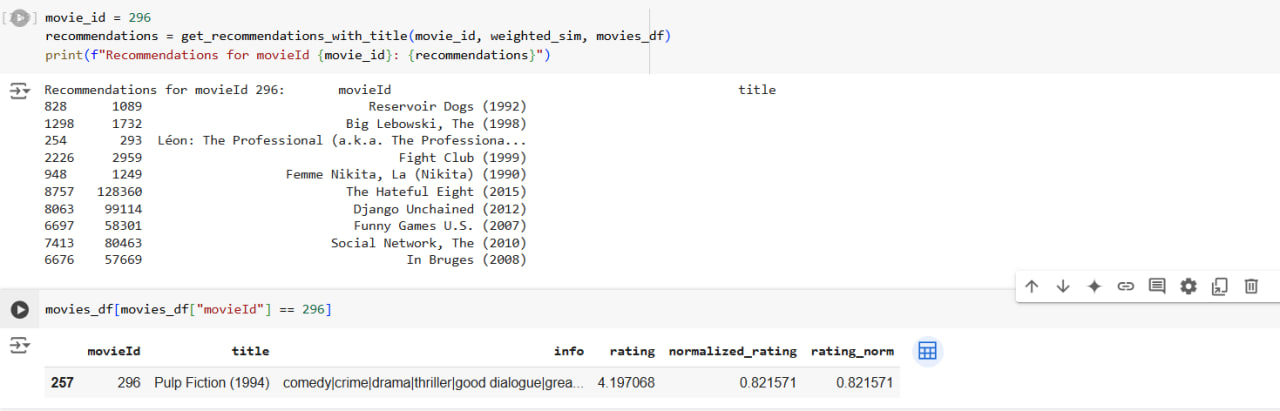
\includegraphics{pic1.png}
\caption{Рекомендации к Pulp Fiction}
\end{figure}

\begin{enumerate}
\def\labelenumi{\arabic{enumi}.}
\item
  \textbf{Исходный фильм}: В данном примере пользователем выбран фильм с
  \texttt{movieId\ =\ 296}, что соответствует фильму \emph{Pulp Fiction
  (1994)}, как видно из таблицы ниже.
\item
  \textbf{Список рекомендаций}: Для оценки релевантности рекомендаций
  можно рассмотреть предложенные фильмы:

  \begin{itemize}
  \tightlist
  \item
    \textbf{Reservoir Dogs (1992)} --- режиссером этого фильма, как и
    \emph{Pulp Fiction}, является Квентин Тарантино, что делает его
    релевантной рекомендацией для фанатов стиля этого режиссера.
  \item
    \textbf{The Big Lebowski (1998)} --- культовый фильм с элементами
    черного юмора и необычным повествованием. Хотя он не от того же
    режиссера, но схож с \emph{Pulp Fiction} по тональности и подходу к
    диалогам.
  \item
    \textbf{Léon: The Professional (1994)} --- еще один культовый фильм
    1990-х с напряженным сюжетом, сильными персонажами и отличной
    драматической составляющей. Хорошо дополняет список для любителей
    криминальных драм.
  \item
    \textbf{Fight Club (1999)} --- фильм с глубоким философским
    подтекстом, сложной сюжетной структурой и культом стиля 90-х. Вполне
    релевантен.
  \item
    \textbf{La Femme Nikita (1990)} --- фильм о криминальной среде, с
    напряженной драмой, который имеет схожие элементы с \emph{Pulp
    Fiction}.
  \item
    \textbf{The Hateful Eight (2015)} --- фильм от того же режиссера
    (Квентин Тарантино), что напрямую делает его релевантным для
    фанатов.
  \item
    \textbf{Django Unchained (2012)} --- еще один фильм Тарантино с
    уникальным стилем повествования, юмором и криминальной драмой, что
    делает его идеально подходящим.
  \item
    \textbf{Funny Games U.S. (2007)} --- психологический триллер,
    который менее связан с \emph{Pulp Fiction}, но может понравиться
    любителям напряженного и мрачного кинематографа.
  \item
    \textbf{The Social Network (2010)} --- рекомендация менее
    релевантна, поскольку это больше биографическая драма о
    технологическом стартапе, а не криминальная драма.
  \item
    \textbf{In Bruges (2008)} --- черная комедия с сильным криминальным
    сюжетом и необычными персонажами, что делает ее очень подходящей
    рекомендацией.
  \end{itemize}
\end{enumerate}

\hypertarget{ux438ux442ux43eux433}{%
\subparagraph{Итог:}\label{ux438ux442ux43eux433}}

Большинство рекомендаций можно считать весьма релевантными, особенно те,
которые связаны с фильмами Квентина Тарантино (\emph{Reservoir Dogs},
\emph{The Hateful Eight}, \emph{Django Unchained}), а также культовые
криминальные драмы и фильмы с черным юмором (\emph{In Bruges},
\emph{Fight Club}). Некоторые фильмы, такие как \emph{The Social
Network}, могут быть менее подходящими в этом контексте, но их включение
может быть связано с особенностями модели (например, схожими ключевыми
словами).

\begin{figure}[H]
\centering
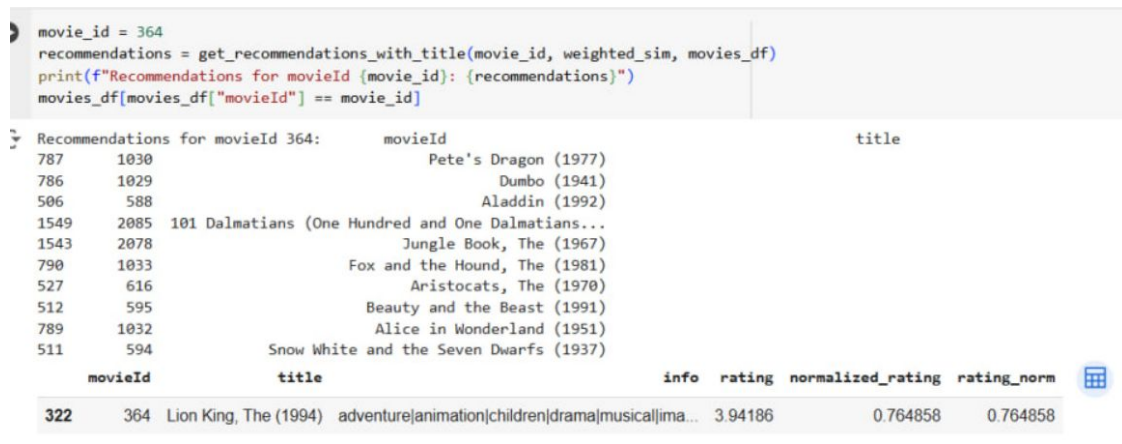
\includegraphics{pic2.png}
\caption{Рекомендации к Lion King}
\end{figure}

\hypertarget{ux43eux446ux435ux43dux43aux430-ux440ux435ux43aux43eux43cux435ux43dux434ux430ux446ux438ux439-ux434ux43bux44f-ux444ux438ux43bux44cux43cux430-the-lion-king-1994}{%
\subsubsection*{\texorpdfstring{Оценка рекомендаций для фильма \emph{The
Lion King
(1994)}}{Оценка рекомендаций для фильма The Lion King (1994)}}\label{ux43eux446ux435ux43dux43aux430-ux440ux435ux43aux43eux43cux435ux43dux434ux430ux446ux438ux439-ux434ux43bux44f-ux444ux438ux43bux44cux43cux430-the-lion-king-1994}}

\begin{enumerate}
\def\labelenumi{\arabic{enumi}.}
\item
  \textbf{Исходный фильм}: В примере используется фильм \emph{The Lion
  King (1994)}, жанры которого включают ``приключения'', ``анимация'',
  ``детский'', ``драма'', ``мюзикл'', ``воображение''.
\item
  \textbf{Список рекомендаций}:

  \begin{itemize}
  \tightlist
  \item
    \textbf{Pete's Dragon (1977)} --- семейный фильм с элементами
    приключений и фантазии, что соответствует жанрам \emph{The Lion
    King}. Рекомендация релевантна.
  \item
    \textbf{Dumbo (1941)} --- анимационный фильм Disney, ориентированный
    на детей, с трогательной сюжетной линией. Подходит к характеристикам
    исходного фильма.
  \item
    \textbf{Aladdin (1992)} --- анимационный мюзикл Disney с
    приключениями и элементами воображения. Очень релевантен как по
    жанрам, так и по стилю.
  \item
    \textbf{101 Dalmatians (1961)} --- классический фильм Disney с
    акцентом на приключения и детей. Хорошо сочетается с \emph{The Lion
    King}.
  \item
    \textbf{The Jungle Book (1967)} --- фильм, связанный с темами
    природы, приключений и животных. Практически идеальная рекомендация.
  \item
    \textbf{The Fox and the Hound (1981)} --- трогательная история о
    дружбе животных, которая перекликается с эмоциональными темами
    \emph{The Lion King}. Рекомендация весьма релевантна.
  \item
    \textbf{The Aristocats (1970)} --- анимационный фильм о
    приключениях, ориентированный на детей. Тематически близок и
    релевантен.
  \item
    \textbf{Beauty and the Beast (1991)} --- анимационный мюзикл Disney
    с драматической сюжетной линией. Очень релевантная рекомендация.
  \item
    \textbf{Alice in Wonderland (1951)} --- приключения в мире фантазий,
    схожи с элементами воображения \emph{The Lion King}. Рекомендация
    уместна.
  \item
    \textbf{Snow White and the Seven Dwarfs (1937)} --- первый
    анимационный фильм Disney, с похожими элементами сказочной драмы и
    мюзикла. Подходит как тематически, так и стилистически.
  \end{itemize}
\end{enumerate}

\hypertarget{ux438ux442ux43eux433-1}{%
\subparagraph{Итог:}\label{ux438ux442ux43eux433-1}}

Все предложенные фильмы можно считать высоко релевантными, поскольку они
либо принадлежат студии Disney, либо имеют схожие жанровые
характеристики, такие как ``анимация'', ``приключения'', ``детский'',
``мюзикл''. Модель демонстрирует отличные результаты в подборе
рекомендаций, соответствующих запросу.

\begin{figure}[H]
\centering
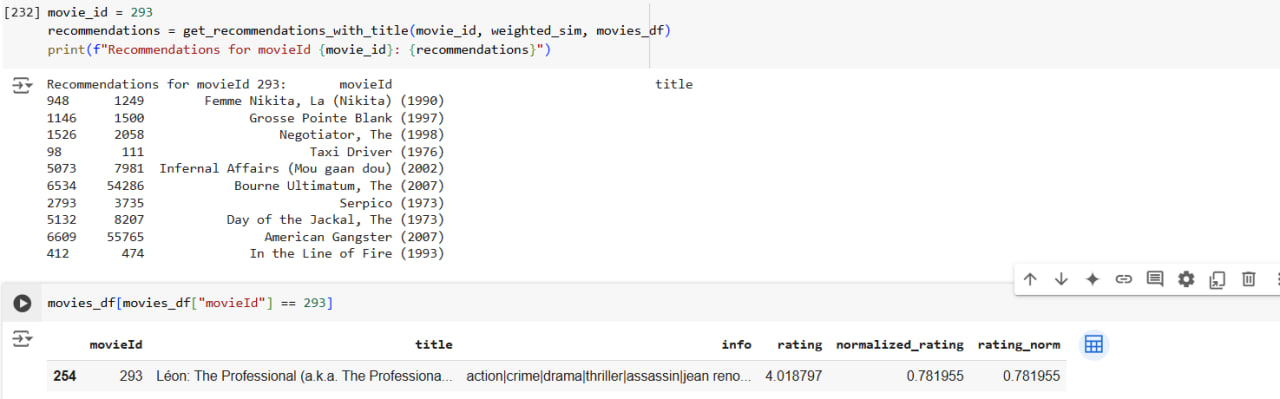
\includegraphics{pic3.png}
\caption{Рекомендации к Leon: The Professional}
\end{figure}

\hypertarget{ux43eux446ux435ux43dux43aux430-ux440ux435ux43aux43eux43cux435ux43dux434ux430ux446ux438ux439-ux434ux43bux44f-ux444ux438ux43bux44cux43cux430-luxe9on-the-professional-1994}{%
\subsubsection*{\texorpdfstring{Оценка рекомендаций для фильма
\emph{Léon: The Professional
(1994)}}{Оценка рекомендаций для фильма Léon: The Professional (1994)}}\label{ux43eux446ux435ux43dux43aux430-ux440ux435ux43aux43eux43cux435ux43dux434ux430ux446ux438ux439-ux434ux43bux44f-ux444ux438ux43bux44cux43cux430-luxe9on-the-professional-1994}}

\begin{enumerate}
\def\labelenumi{\arabic{enumi}.}
\item
  \textbf{Исходный фильм}: В примере используется фильм \emph{Léon: The
  Professional (1994)}
\item
  \textbf{Список рекомендаций}:

  \begin{itemize}
  \tightlist
  \item
    \textbf{Femme Nikita, La (1990)} --- фильм о наемной убийце с
    напряженным драматическим сюжетом. Очень схож по тематике и стилю с
    \emph{Léon}. Рекомендация релевантна.
  \item
    \textbf{Grosse Pointe Blank (1997)} --- черная комедия с элементами
    боевика о профессиональном убийце. Хотя этот фильм более легкий по
    настроению, он пересекается с темой профессиональных убийц.
    Рекомендация умеренно релевантна.
  \item
    \textbf{The Negotiator (1998)} --- напряженный триллер с
    криминальной сюжетной линией и динамичным действием. Отличный выбор
    для поклонников \emph{Léon}. Рекомендация релевантна.
  \item
    \textbf{Taxi Driver (1976)} --- культовый триллер-драма о социально
    отчужденном человеке с элементами насилия и напряжения. Идеально
    подходит как рекомендация по настроению и стилю.
  \item
    \textbf{Infernal Affairs (2002)} --- криминальная драма о мафиози и
    полицейских. Схожий напряженный тон и глубокая драма. Рекомендация
    уместна.
  \item
    \textbf{The Bourne Ultimatum (2007)} --- боевик с акцентом на
    шпионскую тему и динамику. Несмотря на отличие в жанре, фильм
    перекликается с \emph{Léon} элементами боевика. Рекомендация
    умеренно релевантна.
  \item
    \textbf{Serpico (1973)} --- напряженная криминальная драма о борьбе
    с коррупцией в полиции. Хотя здесь нет профессиональных убийц, фильм
    подходит для поклонников криминального жанра. Рекомендация условно
    релевантна.
  \item
    \textbf{Day of the Jackal (1973)} --- триллер о наемном убийце с
    продуманным сюжетом. Очень близко по теме к \emph{Léon}.
    Рекомендация релевантна.
  \item
    \textbf{American Gangster (2007)} --- криминальная драма,
    сосредоточенная на мафиози и преступном мире. Фильм схож жанрово, но
    не столь близок по сюжету. Рекомендация умеренно релевантна.
  \item
    \textbf{In the Line of Fire (1993)} --- триллер о защите президента,
    с элементами криминального жанра. Сюжетно не так близок, но может
    быть интересен любителям напряженных историй. Умеренно релевантно.
  \end{itemize}
\end{enumerate}

\hypertarget{ux438ux442ux43eux433-2}{%
\subparagraph{Итог:}\label{ux438ux442ux43eux433-2}}

Рекомендации в целом достаточно релевантны исходному фильму, особенно
такие фильмы, как \emph{Femme Nikita, La (1990)}, \emph{Taxi Driver
(1976)}, \emph{Day of the Jackal (1973)} и \emph{The Negotiator (1998)}.
Они разделяют ключевые элементы с \emph{Léon}, такие как криминальный
мир, напряжение и сильные персонажи. Менее релевантными выглядят фильмы
вроде \emph{The Bourne Ultimatum} и \emph{In the Line of Fire}, которые
отличаются по тематике и жанру, но все равно могут быть интересны
поклонникам криминальных драм и боевиков.

\hypertarget{ux441ux440ux430ux432ux43dux435ux43dux438ux435-ux43cux43eux434ux435ux43bux435ux439}{%
\subsection*{Сравнение
моделей}\label{ux441ux440ux430ux432ux43dux435ux43dux438ux435-ux43cux43eux434ux435ux43bux435ux439}}


\resizebox{\linewidth}{!}{%
\begin{tabular}{|>{\raggedright\arraybackslash}p{0.12\linewidth}|>{\raggedright\arraybackslash}p{0.18\linewidth}|>{\raggedright\arraybackslash}p{0.50\linewidth}|>{\raggedright\arraybackslash}p{0.10\linewidth}|>{\raggedright\arraybackslash}p{0.10\linewidth}|}
\hline
Модель & Применение & Преимущества & Метрика & Результат \\
\hline
\textbf{UserKNN} & Персональные рекомендации & Высокая точность для активных пользователей; учитывает реальное поведение & NDCG@10 & \textbf{0.8465} \\
\hline
\textbf{Content-based} & Поиск и связанные фильмы & Решает задачу поиска и рекомендации схожих фильмов; подходит для новых пользователей & Ручная проверка & Высокая релевантность \\
\hline
\end{tabular}%
}

\hypertarget{ux43fux43eux447ux435ux43cux443-ux438ux43cux435ux43dux43dux43e-ux44dux442ux438-ux43fux43eux434ux445ux43eux434ux44b}{%
\subsection*{Почему именно эти
подходы?}\label{ux43fux43eux447ux435ux43cux443-ux438ux43cux435ux43dux43dux43e-ux44dux442ux438-ux43fux43eux434ux445ux43eux434ux44b}}

\begin{enumerate}
\def\labelenumi{\arabic{enumi}.}
\tightlist
\item
  \textbf{UserKNN}:

  \begin{itemize}
  \tightlist
  \item
    Эффективен для персонализированных рекомендаций, так как учитывает
    историю оценок пользователей.
  \item
    Метрика NDCG@10 подтверждает, что модель формирует релевантные и
    полезные списки рекомендаций.
  \end{itemize}
\item
  \textbf{Content-based}:

  \begin{itemize}
  \tightlist
  \item
    Необходим для задач поиска, так как позволяет находить фильмы,
    схожие с заданным.
  \item
    Учитывает только содержимое фильмов, что делает модель независимой
    от пользовательских данных.
  \end{itemize}
\end{enumerate}

\hypertarget{ux432ux44bux432ux43eux434ux44b}{%
\subsection*{Выводы}\label{ux432ux44bux432ux43eux434ux44b}}

\begin{itemize}
\tightlist
\item
  \textbf{UserKNN} показал себя как высокоэффективная модель для
  формирования персонализированных рекомендаций. Метрика NDCG@10
  подтверждает качество списка рекомендаций.
\item
  \textbf{Content-based} --- ключевое решение для задач поиска и
  формирования рекомендаций к конкретному фильму. Она позволяет гибко
  учитывать содержание фильмов, обеспечивая высокую релевантность.
\end{itemize}

\endinput